\documentclass[usenames,dvipsnames,tikz]{standalone}
\usepackage{amsmath,amssymb}
\usepackage{xcolor}
\colorlet{tBlue}{RoyalBlue!35!Cerulean}
\colorlet{tRed}{Red}
\usepackage{tikz}
\usepackage{standalone}
\begin{document}
	
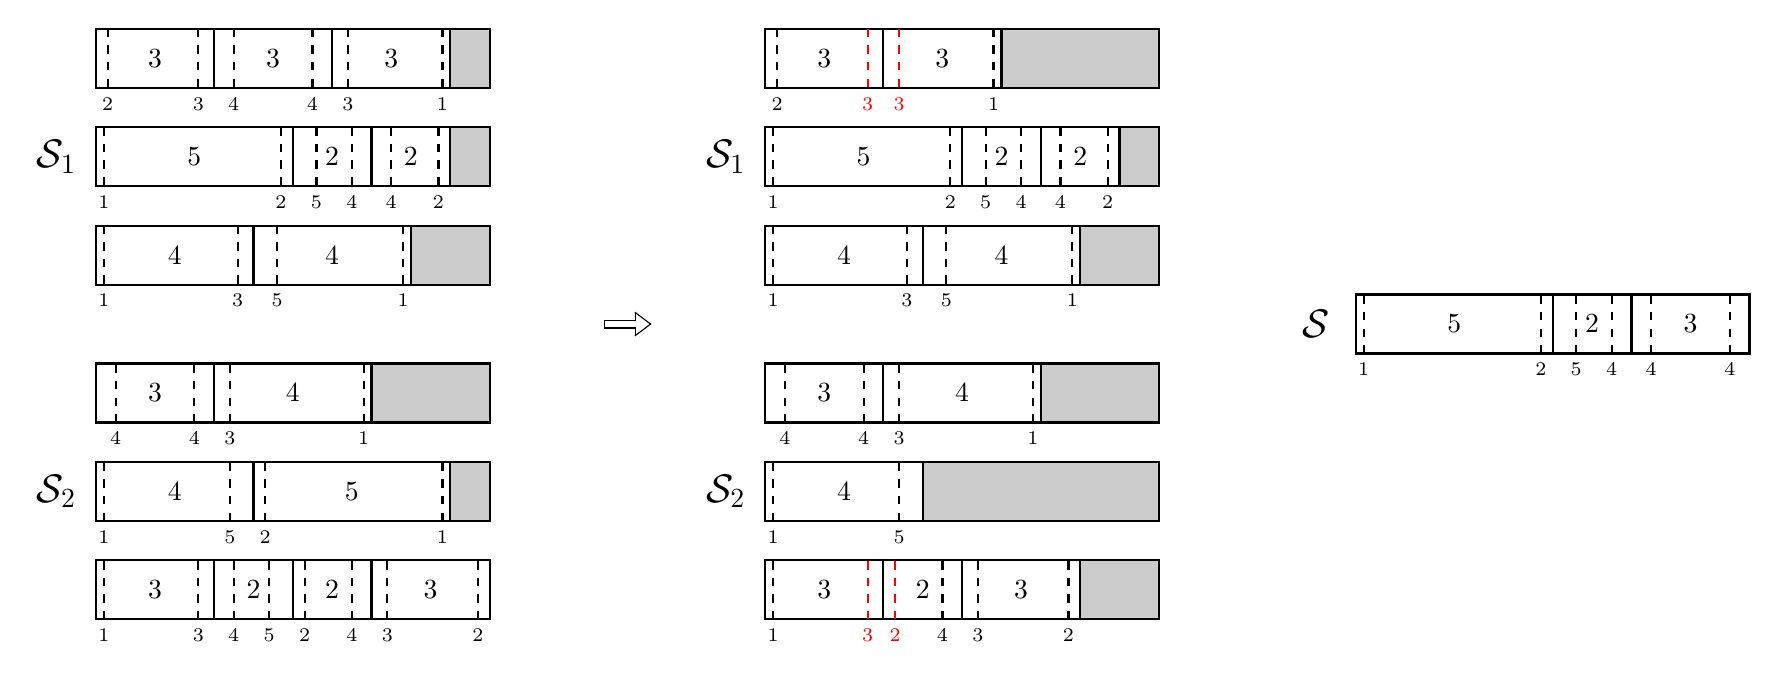
\begin{tikzpicture}
%\draw [help lines] (-1,-2) grid (22,10);
% 1=0.1, 2=0.15, 3=0.2, 4=0.25, 5=0.3
%A=2,(2-4), B=2,(4-5), C=3,(1-3), D=3,(2-3), E=3,(4-4), F=4(1-3), G=4(1-5), H=5(1-2)

%Parent 1 BEFORE
\node at (-0.5, 5.875) {\Large{$\mathcal{S}_1$}};
\draw [thick] (0,4.25) rectangle (5,5);
\draw [thick] (0,5.5) rectangle (5,6.25);
\draw [thick] (0,6.75) rectangle (5,7.5);

%bottom row, 4, 4 (1-3, 5-1) -p1before
\draw [thick] (2,5) -- (2,4.25);
\draw [thick] (4,5) -- (4,4.25);
\filldraw[fill=black!20!white, draw=black, thick] (4,4.25) rectangle (5,5);
\draw [thick, dashed] (0.1,5) -- (0.1,4.25);
\draw [thick, dashed] (1.8,5) -- (1.8,4.25);
\draw [thick, dashed] (2.3,5) -- (2.3,4.25);
\draw [thick, dashed] (3.9,5) -- (3.9,4.25);
\node [below] at (0.1,4.25) {\scriptsize{1}};
\node [below] at (1.8,4.25) {\scriptsize{3}};
\node [below] at (2.3,4.25) {\scriptsize{5}};
\node [below] at (3.9,4.25) {\scriptsize{1}};
\node at (1,4.625) {4};
\node at (3,4.625) {4};
%\node at (1,5.15) {\footnotesize{4}};
%\node at (1,5.5) {G};
%\node at (3,5.15) {\footnotesize{4}};
%\node at (3,5.5) {F};


%middle row, 5, 2, 2 (1-2, 5-4, 4-2) -p1before
\draw [thick] (2.5,6.25) -- (2.5,5.5);
\draw [thick] (3.5,6.25) -- (3.5,5.5);
\filldraw[fill=black!20!white, draw=black, thick] (4.5,5.5) rectangle (5,6.25);
\draw [thick, dashed] (0.1,6.25) -- (0.1,5.5);
\draw [thick, dashed] (2.35,6.25) -- (2.35,5.5);
\draw [thick, dashed] (2.8,6.25) -- (2.8,5.5);
\draw [thick, dashed] (3.25,6.25) -- (3.25,5.5);
\draw [thick, dashed] (3.75,6.25) -- (3.75,5.5);
\draw [thick, dashed] (4.35,6.25) -- (4.35,5.5);
\node [below] at (0.1,5.5) {\scriptsize{1}};
\node [below] at (2.35,5.5) {\scriptsize{2}};
\node [below] at (2.8,5.5) {\scriptsize{5}};
\node [below] at (3.25,5.5) {\scriptsize{4}};
\node [below] at (3.75,5.5) {\scriptsize{4}};
\node [below] at (4.35,5.5) {\scriptsize{2}};
\node at (1.25,5.875) {5};
\node at (3,5.875) {2};
\node at (4,5.875) {2};
%\node at (1.25,6.4) {\footnotesize{5}};
%\node at (1.25,6.75) {H};
%\node at (3,6.4) {\footnotesize{2}};
%\node at (3,6.75) {B};
%\node at (4,6.4) {\footnotesize{2}};
%\node at (4,6.75) {A};


%top row, 3, 3, 3 (2-3, 4-4, 3-1) -p1before
\draw [thick] (1.5,7.5) -- (1.5,6.75);
\draw [thick] (3,7.5) -- (3,6.75);
\draw [thick] (4.5,7.5) -- (4.5,6.75);
\filldraw[fill=black!20!white, draw=black, thick] (4.5,6.75) rectangle (5,7.5);
\draw [thick, dashed] (0.15,7.5) -- (0.15,6.75);
\draw [thick, dashed] (1.3,7.5) -- (1.3,6.75);
\draw [thick, dashed] (1.75,7.5) -- (1.75,6.75);
\draw [thick, dashed] (2.75,7.5) -- (2.75,6.75);
\draw [thick, dashed] (3.2,7.5) -- (3.2,6.75);
\draw [thick, dashed] (4.4,7.5) -- (4.4,6.75);
\node [below] at (0.15,6.75) {\scriptsize{2}};
\node [below] at (1.3,6.75) {\scriptsize{3}};
\node [below] at (1.75,6.75) {\scriptsize{4}};
\node [below] at (2.75,6.75) {\scriptsize{4}};
\node [below] at (3.2,6.75) {\scriptsize{3}};
\node [below] at (4.4,6.75) {\scriptsize{1}};
\node at (0.75,7.125) {3};
\node at (2.25,7.125) {3};
\node at (3.75,7.125) {3};

%-----------------------------------------------------------

%Parent 2 BEFORE
\node at (-0.5,1.625) {\Large{$\mathcal{S}_2$}};
\draw [thick] (0,0) rectangle (5,0.75);
\draw [thick] (0,1.25) rectangle (5,2);
\draw [thick] (0,2.5) rectangle (5,3.25);

%bottom row, 3, 2, 2, 3 (1-3, 4-5, 2-4, 3-2) - p2before
\draw [thick] (1.5,0) -- (1.5,0.75);
\draw [thick] (2.5,0) -- (2.5,0.75);
\draw [thick] (3.5,0) -- (3.5,0.75);
\draw [thick, dashed] (0.1,0) -- (0.1,0.75);
\draw [thick, dashed] (1.3,0) -- (1.3,0.75);
\draw [thick, dashed] (1.75,0) -- (1.75,0.75);
\draw [thick, dashed] (2.2,0) -- (2.2,0.75);
\draw [thick, dashed] (2.65,0) -- (2.65,0.75);
\draw [thick, dashed] (3.25,0) -- (3.25,0.75);
\draw [thick, dashed] (3.7,0) -- (3.7,0.75);
\draw [thick, dashed] (4.85,0) -- (4.85,0.75);
\node [below] at (0.1,0) {\scriptsize{1}};
\node [below] at (1.3,0) {\scriptsize{3}};
\node [below] at (1.75,0) {\scriptsize{4}};
\node [below] at (2.2,0) {\scriptsize{5}};
\node [below] at (2.65,0) {\scriptsize{2}};
\node [below] at (3.25,0) {\scriptsize{4}};
\node [below] at (3.7,0) {\scriptsize{3}};
\node [below] at (4.85,0) {\scriptsize{2}};
\node at (0.75,0.375) {3};
\node at (2,0.375) {2};
\node at (3,0.375) {2};
\node at (4.25,0.375) {3};

%middle row, 4, 5 (1-5, 2-1) - p2before
\draw [thick] (2,1.25) -- (2,2);
\draw [thick] (4.5,1.25) -- (4.5,2);
\filldraw[fill=black!20!white, draw=black, thick] (4.5,1.25) rectangle (5,2);
\draw [thick, dashed] (0.1,1.25) -- (0.1,2);
\draw [thick, dashed] (1.7,1.25) -- (1.7,2);
\draw [thick, dashed] (2.15,1.25) -- (2.15,2);
\draw [thick, dashed] (4.4,1.25) -- (4.4,2);
\node [below] at (0.1,1.25) {\scriptsize{1}};
\node [below] at (1.7,1.25) {\scriptsize{5}};
\node [below] at (2.15,1.25) {\scriptsize{2}};
\node [below] at (4.4,1.25) {\scriptsize{1}};
\node at (1,1.625) {4};
\node at (3.25,1.625) {5};

%top row, 3, 4 (4-4, 3-1) - p2before
\draw [thick] (1.5,2.5) -- (1.5,3.25);
\draw [thick] (3.5,2.5) -- (3.5,3.25);
\filldraw[fill=black!20!white, draw=black, thick] (3.5,2.5) rectangle (5,3.25);
\draw [thick, dashed] (0.25,2.5) -- (0.25,3.25);
\draw [thick, dashed] (1.25,2.5) -- (1.25,3.25);
\draw [thick, dashed] (1.7,2.5) -- (1.7,3.25);
\draw [thick, dashed] (3.4,2.5) -- (3.4,3.25);
\node [below] at (0.25,2.5) {\scriptsize{4}};
\node [below] at (1.25,2.5) {\scriptsize{4}};
\node [below] at (1.7,2.5) {\scriptsize{3}};
\node [below] at (3.4,2.5) {\scriptsize{1}};
\node at (0.75,2.875) {3};
\node at (2.5,2.875) {4};

%-----------------------------------
\draw (6.45,3.7) -- (6.85,3.7);
\draw (6.45,3.8) -- (6.85,3.8);
\draw (7.05,3.745) -- (6.845,3.9);
\draw (7.05,3.755) -- (6.845,3.6);
\draw (6.85,3.9) -- (6.85,3.79);
\draw (6.85,3.6) -- (6.85,3.71);
\draw (6.46,3.7) -- (6.46,3.8);

%AFTER ITEMS REMOVED %%%%%%%%%%%%%%%%%%%%%%%%%%%%%%%%%%%%%%%%%%%%%%%%%%%%%%%

%Parent 1 AFTER
\node at (8, 5.875) {\Large{$\mathcal{S}_1$}};
\draw [thick] (8.5,4.25) rectangle (13.5,5);
\draw [thick] (8.5,5.5) rectangle (13.5,6.25);
\draw [thick] (8.5,6.75) rectangle (13.5,7.5);

%bottom row, 4, 4 (1-3, 5-1) -p1after
\draw [thick] (10.5,5) -- (10.5,4.25);
\draw [thick] (12.5,5) -- (12.5,4.25);
\filldraw[fill=black!20!white, draw=black, thick] (12.5,4.25) rectangle (13.5,5);
\draw [thick, dashed] (8.6,5) -- (8.6,4.25);
\draw [thick, dashed] (10.3,5) -- (10.3,4.25);
\draw [thick, dashed] (10.8,5) -- (10.8,4.25);
\draw [thick, dashed] (12.4,5) -- (12.4,4.25);
\node [below] at (8.6,4.25) {\scriptsize{1}};
\node [below] at (10.3,4.25) {\scriptsize{3}};
\node [below] at (10.8,4.25) {\scriptsize{5}};
\node [below] at (12.4,4.25) {\scriptsize{1}};
\node at (9.5,4.625) {4};
\node at (11.5,4.625) {4};

%middle row, 5, 2, 2 (1-2, 5-4, 4-2) p1after
\draw [thick] (11,6.25) -- (11,5.5);
\draw [thick] (12,6.25) -- (12,5.5);
\draw [thick] (13,6.25) -- (13,5.5);
\filldraw[fill=black!20!white, draw=black, thick] (13,5.5) rectangle (13.5,6.25);
\draw [thick, dashed] (8.6,6.25) -- (8.6,5.5);
\draw [thick, dashed] (10.85,6.25) -- (10.85,5.5);
\draw [thick, dashed] (11.3,6.25) -- (11.3,5.5);
\draw [thick, dashed] (11.75,6.25) -- (11.75,5.5);
\draw [thick, dashed] (12.25,6.25) -- (12.25,5.5);
\draw [thick, dashed] (12.85,6.25) -- (12.85,5.5);
\node [below] at (8.6,5.5) {\scriptsize{1}};
\node [below] at (10.85,5.5) {\scriptsize{2}};
\node [below] at (11.3,5.5) {\scriptsize{5}};
\node [below] at (11.75,5.5) {\scriptsize{4}};
\node [below] at (12.25,5.5) {\scriptsize{4}};
\node [below] at (12.85,5.5) {\scriptsize{2}};
\node at (9.75,5.875) {5};
\node at (11.5,5.875) {2};
\node at (12.5,5.875) {2};

%CHANGED - top row, 3, 3 (2-3 X 3-1) (removed middle item, vsc violated) - p1after
\draw [thick] (10,7.5) -- (10,6.75);
\draw [thick] (11.5,7.5) -- (11.5,6.75);
\filldraw[fill=black!20!white, draw=black, thick] (11.5,6.75) rectangle (13.5,7.5);
\draw [thick, dashed] (8.65,7.5) -- (8.65,6.75);
\draw [thick, dashed, tRed] (9.8,7.5) -- (9.8,6.75);
\draw [thick, dashed, tRed] (10.2,7.5) -- (10.2,6.75);
\draw [thick, dashed] (11.4,7.5) -- (11.4,6.75);
\node [below] at (8.65,6.75) {\scriptsize{2}};
\node [below] at (9.8,6.75) {\textcolor{tRed}{\scriptsize{3}}};
\node [below] at (10.2,6.75) {\textcolor{tRed}{\scriptsize{3}}};
\node [below] at (11.4,6.75) {\scriptsize{1}};
\node at (9.25,7.125) {3};
\node at (10.75,7.125) {3};

%---------------------------------------------

%Parent 2 AFTER
\node at (8,1.625) {\Large{$\mathcal{S}_2$}};
\draw [thick] (8.5,0) rectangle (13.5,0.75);
\draw [thick] (8.5,1.25) rectangle (13.5,2);
\draw [thick] (8.5,2.5) rectangle (13.5,3.25);

%CHANGED - bottom row, 3, 2, 3 (1-3 X 2-4, 3-2) (removed second item, vsc violated) - p2after
\draw [thick] (10,0) -- (10,0.75);
\draw [thick] (11,0) -- (11,0.75);
\draw [thick] (12.5,0) -- (12.5,0.75);
\filldraw[fill=black!20!white, draw=black, thick] (12.5,0) rectangle (13.5,0.75);
\draw [thick, dashed] (8.6,0) -- (8.6,0.75);
\draw [thick, dashed, tRed] (9.8,0) -- (9.8,0.75);
\draw [thick, dashed, tRed] (10.15,0) -- (10.15,0.75);
\draw [thick, dashed] (10.75,0) -- (10.75,0.75);
\draw [thick, dashed] (11.2,0) -- (11.2,0.75);
\draw [thick, dashed] (12.35,0) -- (12.35,0.75);
\node [below] at (8.6,0) {\scriptsize{1}};
\node [below] at (9.8,0) {\textcolor{tRed}{\scriptsize{3}}};
\node [below] at (10.15,0) {\textcolor{tRed}{\scriptsize{2}}};
\node [below] at (10.75,0) {\scriptsize{4}};
\node [below] at (11.2,0) {\scriptsize{3}};
\node [below] at (12.35,0) {\scriptsize{2}};
\node at (9.25,0.375) {3};
\node at (10.5,0.375) {2};
\node at (11.75,0.375) {3};


%CHANGED - middle row, 4 (1-5) (removed last item) - p2after
\draw [thick] (10.5,1.25) -- (10.5,2);
\filldraw[fill=black!20!white, draw=black, thick] (10.5,1.25) rectangle (13.5,2);
\draw [thick, dashed] (8.6,1.25) -- (8.6,2);
\draw [thick, dashed] (10.2,1.25) -- (10.2,2);
\node [below] at (8.6,1.25) {\scriptsize{1}};
\node [below] at (10.2,1.25) {\scriptsize{5}};
\node at (9.5,1.625) {4};

%top row, 3, 4 (4-4, 3-1) - p2after
\draw [thick] (10,2.5) -- (10,3.25);
\draw [thick] (12,2.5) -- (12,3.25);
\filldraw[fill=black!20!white, draw=black, thick] (12,2.5) rectangle (13.5,3.25);
\draw [thick, dashed] (8.75,2.5) -- (8.75,3.25);
\draw [thick, dashed] (9.75,2.5) -- (9.75,3.25);
\draw [thick, dashed] (10.2,2.5) -- (10.2,3.25);
\draw [thick, dashed] (11.9,2.5) -- (11.9,3.25);
\node [below] at (8.75,2.5) {\scriptsize{4}};
\node [below] at (9.75,2.5) {\scriptsize{4}};
\node [below] at (10.2,2.5) {\scriptsize{3}};
\node [below] at (11.9,2.5) {\scriptsize{1}};
\node at (9.25,2.875) {3};
\node at (11,2.875) {4};

%---------------------------------------------
% OFFSPRING
\node at (15.5,3.75) {\Large{$\mathcal{S}$}};

% items 5, 2, 3 (1-2, 5-4, 4-4)
\draw [thick] (16,3.375) rectangle (21,4.125);
\draw [thick] (18.5,3.375) -- (18.5,4.125);
\draw [thick] (19.5,3.375) -- (19.5,4.125);

\draw [thick, dashed] (16.1,3.375) -- (16.1,4.125);
\draw [thick, dashed] (18.35, 3.375) -- (18.35,4.125);
\draw [thick, dashed] (18.8,3.375) -- (18.8,4.125);
\draw [thick, dashed] (19.25,3.375) -- (19.25,4.125);
\draw [thick, dashed] (19.75, 3.375) -- (19.75,4.125);
\draw [thick, dashed] (20.75,3.375) -- (20.75,4.125);
\node [below] at (16.1,3.375) {\scriptsize{1}};
\node [below] at (18.35,3.375) {\scriptsize{2}};
\node [below] at (18.8,3.375) {\scriptsize{5}};
\node [below] at (19.25,3.375) {\scriptsize{4}};
\node [below] at (19.75,3.375) {\scriptsize{4}};
\node [below] at (20.75,3.375) {\scriptsize{4}};

\node at (17.25,3.75) {5};
\node at (19,3.75) {2};
\node at (20.25,3.75) {3};



\end{tikzpicture}
	
\end{document}